\documentclass[review, doubleblind, 3p,
authoryear]{elsarticle} %review=doublespace preprint=single 5p=2 column
%%% Begin My package additions %%%%%%%%%%%%%%%%%%%

\usepackage[hyphens]{url}

  \journal{Computers, Environment and Urban Studies} % Sets Journal name

\usepackage{graphicx}
%%%%%%%%%%%%%%%% end my additions to header

\usepackage[T1]{fontenc}
\usepackage{lmodern}
\usepackage{amssymb,amsmath}
% TODO: Currently lineno needs to be loaded after amsmath because of conflict
% https://github.com/latex-lineno/lineno/issues/5
\usepackage{lineno} % add
  \linenumbers % turns line numbering on
\usepackage{ifxetex,ifluatex}
\usepackage{fixltx2e} % provides \textsubscript
% use upquote if available, for straight quotes in verbatim environments
\IfFileExists{upquote.sty}{\usepackage{upquote}}{}
\ifnum 0\ifxetex 1\fi\ifluatex 1\fi=0 % if pdftex
  \usepackage[utf8]{inputenc}
\else % if luatex or xelatex
  \usepackage{fontspec}
  \ifxetex
    \usepackage{xltxtra,xunicode}
  \fi
  \defaultfontfeatures{Mapping=tex-text,Scale=MatchLowercase}
  \newcommand{\euro}{€}
\fi
% use microtype if available
\IfFileExists{microtype.sty}{\usepackage{microtype}}{}

\ifxetex
  \usepackage[setpagesize=false, % page size defined by xetex
              unicode=false, % unicode breaks when used with xetex
              xetex]{hyperref}
\else
  \usepackage[unicode=true]{hyperref}
\fi
\hypersetup{breaklinks=true,
            bookmarks=true,
            pdfauthor={},
            pdftitle={biclaR: Estimating the socio-environmental impacts of car substitution by bicycle and public transit using open tools},
            colorlinks=true,
            urlcolor=blue,
            linkcolor=blue,
            pdfborder={0 0 0}}

\setcounter{secnumdepth}{5}
% Pandoc toggle for numbering sections (defaults to be off)


% tightlist command for lists without linebreak
\providecommand{\tightlist}{%
  \setlength{\itemsep}{0pt}\setlength{\parskip}{0pt}}


% Pandoc citation processing
\newlength{\cslhangindent}
\setlength{\cslhangindent}{1.5em}
\newlength{\csllabelwidth}
\setlength{\csllabelwidth}{3em}
\newlength{\cslentryspacingunit} % times entry-spacing
\setlength{\cslentryspacingunit}{\parskip}
% for Pandoc 2.8 to 2.10.1
\newenvironment{cslreferences}%
  {}%
  {\par}
% For Pandoc 2.11+
\newenvironment{CSLReferences}[2] % #1 hanging-ident, #2 entry spacing
 {% don't indent paragraphs
  \setlength{\parindent}{0pt}
  % turn on hanging indent if param 1 is 1
  \ifodd #1
  \let\oldpar\par
  \def\par{\hangindent=\cslhangindent\oldpar}
  \fi
  % set entry spacing
  \setlength{\parskip}{#2\cslentryspacingunit}
 }%
 {}
\usepackage{calc}
\newcommand{\CSLBlock}[1]{#1\hfill\break}
\newcommand{\CSLLeftMargin}[1]{\parbox[t]{\csllabelwidth}{#1}}
\newcommand{\CSLRightInline}[1]{\parbox[t]{\linewidth - \csllabelwidth}{#1}\break}
\newcommand{\CSLIndent}[1]{\hspace{\cslhangindent}#1}


\usepackage{subfig}
\usepackage{booktabs}
\usepackage{longtable}
\usepackage{array}
\usepackage{multirow}
\usepackage{wrapfig}
\usepackage{float}
\usepackage{colortbl}
\usepackage{pdflscape}
\usepackage{tabu}
\usepackage{threeparttable}
\usepackage{threeparttablex}
\usepackage[normalem]{ulem}
\usepackage{makecell}
\usepackage{xcolor}

\biboptions{authoryear}
\usepackage{url}
\usepackage{float}
\usepackage{booktabs}
\usepackage{longtable}
\usepackage{makecell}
\usepackage{multirow}

\begin{document}


\begin{frontmatter}

  \title{biclaR: Estimating the socio-environmental impacts of car
substitution by bicycle and public transit using open tools}
    \author[CERIS]{Rosa Félix\corref{cor1}%
  \corref{cor1}%
  }
   \ead{rosamfelix@tecnico.ulisboa.pt} 
    \author[CERIS]{Filipe Moura%
  %
  }
   \ead{fmoura@tecnico.ulisboa.pt} 
    \author[ITS]{Robin Lovelace%
  %
  }
   \ead{r.lovelace@uleeds.uk} 
      \affiliation[CERIS]{CERIS, Instituto Superior Técnico -
Universidade de Lisboa, Av Rovisco Pais 1, 1049-001 Lisboa, Portugal}
    \affiliation[ITS]{Institute for Transport Studies, University of
Leeds. 34-40 University Rd, Leeds LS2 9JT, UK}
    \cortext[cor1]{Corresponding author}
  
  \begin{abstract}
  A high proportion of car trips can be replaced by a combination of
  public transit and cycling for the first-and-last mile. This paper
  estimates the potential for cycling combined with public transit (PT)
  as a substitute for car trips in the Lisbon metropolitan area and
  assesses its socio-environmental impacts using open data and open
  source tools. A decision support tool that facilitates the design and
  development of a metropolitan cycling network was developed
  (\emph{biclaR}). The social and environmental impacts were assessed
  using the \emph{HEAT for Cycling} and the \emph{HEAT as a Service}
  tools. The impacts of shifting car trips to PT were also estimated and
  monetized. The results indicate that 10\% of trips could be made by
  bicycle + PT combination. Shifting to cycling for the first-and-last
  mile stages can reduce annual CO\textsubscript{2}eq emissions from
  6,000 tons/day, with benefits over 10 years of at least €230 million.
  For the PT leg, the transfer from car avoids of up to 20,500 tons of
  CO\textsubscript{2}eq emissions per year. This evidence can support
  policymakers to prioritize interventions that reduce the reliance on
  private motor vehicles.\\
  \end{abstract}
    \begin{keyword}
    Active transport \sep Intermodality \sep First and last
mile \sep Health economic assessment \sep Environmental impacts \sep 
    Open data and methods
  \end{keyword}
  
 \end{frontmatter}

\hypertarget{introduction}{%
\section{Introduction}\label{introduction}}

Combining public transportation (PT) and cycling for the first and last
mile in metropolitan areas can significantly replace private car trips
(Martens, 2007; Rietveld, 2000). This approach requires interventions
and programs to make bicycling more appealing, and the resulting public
investments can have significant social and environmental benefits.

According to the latest mobility survey conducted in 2018 (INE, 2018),
the LMA registered a total of 5.3 million daily trips, with only 0.5\%
by bicycle. Car modal share was 58.4\%, while PT accounted for 15.5\%.
The number of intra-municipal trips --- with origin and destination in
the same municipality --- amounts to 3.5 million trips. This exceeds the
number of inter-municipal trips (1.8 million trips), involving travel
between different municipalities. Cars and public transport are the most
used modes for intercity trips, with cars being the predominant choice
for all journeys.

To achieve the cycling targets set by the Portuguese national cycling
strategy for 2025 and 2030 (4\% and 10\%, respectively) (Presidência do
Conselho de Ministros, 2019), the Lisbon's Metropolitan Department of
Transport introduced \emph{biclaR}\footnote{See
  \href{https://biclar.tmlmobilidade.pt/}{biclar.tmlmobilidade.pt}.}, a
decision support tool that facilitates the planning, design, and
development of a metropolitan cycling network (Félix et al., 2022).

\emph{biclaR} builds on the Propensity to Cycle Tool\footnote{See
  \href{https://www.pct.bike/}{pct.bike}.} (PCT), a web application and
research project funded by the UK's Department for Transport in 2015
which launched nationally in 2017 as part of the government's Cycling
and Walking Investment Strategy. The PCT initially used only
origin-destination data for commuting trips as the basis of estimates of
cycling potential at zone, route and route network levels (Lovelace et
al., 2017). The PCT has been extended to include cycling potential for
travel to school in England (Goodman et al., 2019) and other trip types
in other countries.\footnote{See \href{https://www.npt.scot}{npt.scot}
  and \href{https://cruse.bike}{cruse.bike} for examples of the PCT in
  Scotland and Ireland that include estimates of cycling for other
  purposes.} However, to the best of our knowledge, this is the first
time that the method has been integrated with public transport data
using multi-modal routing to estimate the potential and benefits of
multi-stage cycling and PT trips.

This paper estimates the potential for combining cycling and PT to
substitute car trips in the LMA. After presenting the methods used, it
assesses its socio-environmental impacts using open data and open-source
tools.

\hypertarget{methods}{%
\section{Methods}\label{methods}}

\hypertarget{modeling-origin-destination-trips}{%
\subsection{Modeling Origin-Destination
trips}\label{modeling-origin-destination-trips}}

The mobility survey data (INE, 2018) is the basis for this project and
defines the baseline scenario. Despite being conducted in the
pre-pandemic period (2017), this dataset represents the most
comprehensive and up-to-date information on urban mobility in Portuguese
metropolitan areas (Lisbon and Porto).

We used a method for disaggregating the origins and destinations of
trips between the centroids of two districts (same as ``parish'') to
ensure that a district is not solely characterized by a single point of
origin and destination for its trips. Aggregating all trips into
centroids renders the exercise less realistic, as it excludes a
significant portion of short-distance trips, a prevalent characteristic
of active mode travel (Lovelace et al., 2022b). The OD Jittering method
breaks down a single point (i.e., the centroid of an area) into multiple
random points on the existing and neighboring road network, using
OpenStreetMap as a reference. This method then distributes the volume of
trips within the district among the randomly generated
origin-destination pairs.

Using the
\href{https://github.com/dabreegster/odjitter}{\texttt{odjitter} R
package}, we employed a maximum disaggregation level of 100 trips per
O-D pair for this project. Figure \ref{fig:jitter} illustrates the
contrast between trip representation through the traditional method,
which connects a single desire line between each district, and the
presentation achieved through the randomization and disaggregation of
trips between districts, specifically for the Lisbon metropolitan area.

\begin{figure}

{\centering 
\includegraphics[width=1\linewidth,]{img/jitter} 

}

\caption{Representation of OD pairs in the Lisbon metropolitan area between districts, without jittering (left) and with jittering (right).}\label{fig:jitter}
\end{figure}

Although this method provides a more realistic representation of the
trips undertaken compared to the traditional approach, it does not fully
align with the actual O-D pairs of trips, which remain unknown due to
data privacy regulations.

\hypertarget{modeling-routes}{%
\subsection{Modeling routes}\label{modeling-routes}}

The mobility survey collects the origin and destination of trips but
does not include the respective routes. Modeling the realistic cycling +
PT routes between OD pairs depends on assumptions regarding the
characteristics of the cycling and road networks and the location of
public transport interfaces. Other constraints regarding the behavior of
potential cyclists determine the routing results. For example, such
restrictions can favor low speed, low traffic streets, more direct
routes, and less steep paths, among others, suitable for cycling.

The selected route choice algorithm was the
\href{https://ipeagit.github.io/r5r/}{\texttt{r5r} R package} (Pereira
et al., 2021), which allows for great flexibility in configuring
estimated route types, and which proven to provide most accurate route
networks for the city of Lisbon (Lovelace et al., 2022a). \texttt{r5r}
can calculate multi-modal routes using PT combined with other modes. It
enables the identification of the most direct or safest cycling routes,
using the Level of Traffic Stress\footnote{see
  \href{https://docs.conveyal.com/learn-more/traffic-stress}{docs.conveyal.com/learn-more/traffic-stress}.}
(LTS) scale, ranging from 1 to 4, where 1 corresponds to the quietest
(e.g., off-road cycle paths) and 4 corresponds to the least quiet (e.g.,
routes shared with motorized traffic). The routes were estimated for the
base scenario for both types of networks: \emph{direct} and \emph{safe},
using LTS 4 and LTS 3, respectively. Different routing profiles enable
decision-makers to plan for different bicycle user typologies and/or for
different city cycling maturity levels (Félix et al., 2017).

The \texttt{r5r} model used the OpenStreetMap road network and the GTFS
metropolitan data aggregated and validated. This information is crucial
for an accurate PT trip and route estimation. A digital elevation model,
from the European Space Agency's COPERNICUS mission, was used to include
street gradient information, as a weight in cycling routing. The cycling
potential trips for the two national strategic targets (4\% and 10\%)
were estimated from the 2017 cycling and car trips (both as a driver and
as a passenger), the baseline scenario.

The routes were then overlaid and aggregated by segments, using
\href{https://docs.ropensci.org/stplanr/reference/overline.html}{\texttt{stplanr\ overline()}
R function}.

\hypertarget{modeling-intermodality}{%
\subsection{Modeling intermodality}\label{modeling-intermodality}}

The intermodality scenario considers trips combining PT and cycling for
the first and last legs. In a conservative approach, we have restricted
our analysis to the first and last legs with a combined length of up to
5 km (for instance: 1 km from origin to interface A plus 4 km from
interface B to destination) or up to 25 minutes on bike. Furthermore, we
have imposed restrictions on PT usage to include only trips with no PT
transfers, and up to 2 hours (120 min). Additionally, we have only
included PT modes that can easily accommodate bicycles, such as trains,
ferries, trams, and inter-municipal bus lines equipped with bike racks
(Figure \ref{fig:map1}).

\begin{figure}

{\centering 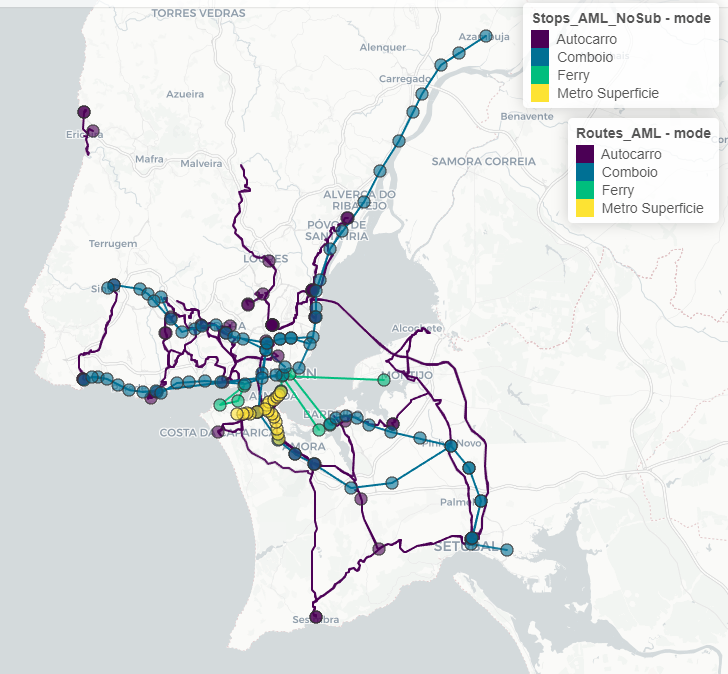
\includegraphics[width=0.6\linewidth,]{img/map1} 

}

\caption{Interfaces and lines considered, by transport mode, in the Lisbon metropolitan area}\label{fig:map1}
\end{figure}

Figure \ref{fig:map2} illustrates the resulting bicycle routes to access
the main PT interfaces in the LMA.

\begin{figure}

{\centering 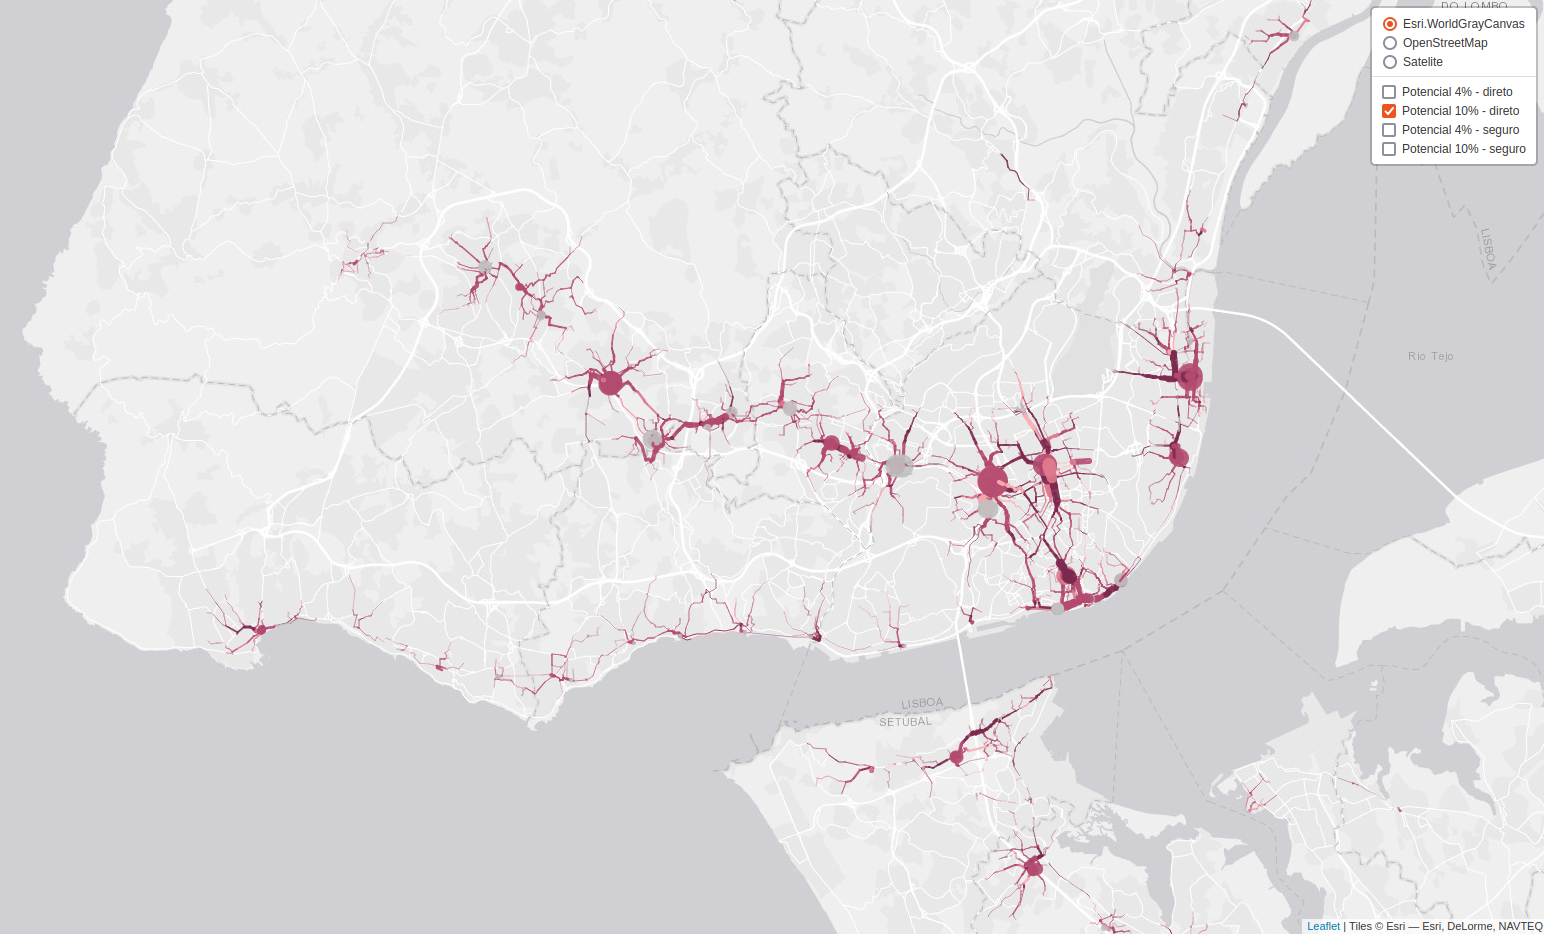
\includegraphics[width=0.8\linewidth,]{img/map2} 

}

\caption{Bike routes with highest potential to serve as first and last leg when replacing cycling and PT from car trips (screenshot of the interactive online tool).}\label{fig:map2}
\end{figure}

\hypertarget{assessing-socio-environmental-benefits}{%
\subsection{Assessing socio-environmental
benefits}\label{assessing-socio-environmental-benefits}}

For the cycling legs of the journey (first and last legs),
socio-environmental impacts were estimated, using the HEAT for Cycling
tool v5.0 (Kahlmeier et al., 2017) from the World Health Organization,
and the
\href{https://github.com/HEAT-WHO/HEAT_heatr_api}{\texttt{HEATaaS} R
package}\footnote{\texttt{HEATaaS} is under development. For more
  information contact
  \href{https://heatwalkingcycling.org}{heatwalkingcycling.org}.}. The
HEAT tool provided estimates on the shifting from car to cycling for a
short term time horizon (i.e., one year) and the long term (i.e., ten
years). We considered two dimensions: \emph{social} --- including the
physical activity of cyclists, air pollution exposure, and road
casualties; \emph{environmental} --- including CO\textsubscript{2}eq
emissions and other pollutants.

For the second leg of the journey, we estimate the additional
environmental impacts of shifting car trips to PT (between the PT
interfaces).

To estimate the car emissions, we used the EMEP/EEA's COPERT software v5
methods and reference values (Ntziachristos \& Samaras, 2020) for a Tier
3 detail level. We used a family-size vehicle, EURO standard, and
gasoline or diesel fuel. All trips were considered to be made under
urban conditions and at an average speed of 15 km/h during rush hour
periods. Since the average distance traveled per trip influences the
overconsumption and emissions from cold-start engine operation, we
estimated energy and emission factors for different ranges of trips at
500-meter intervals. In addition, we assumed an occupancy rate of 1.6
passengers \emph{per} car (INE, 2018).

Regarding PT, we considered the emission factor values reported in the
environmental and sustainability reports of the PT operators in the LMA
(Carris, 2020; CP, 2020; Metropolitano de Lisboa, 2020; Transtejo,
2014).

Emissions were estimated for the following atmospheric pollutants: CO,
PM10, NOx, and VOC; and for the main green house gases:
CO\textsubscript{2}, CH\textsubscript{4}, and N\textsubscript{2}O,
converted in CO\textsubscript{2}eq. In particular, for the urban train
and tram -- with 100\% electric traction -- only CO\textsubscript{2}eq
emissions were considered (resulting from the production of electricity,
considering a ``well-to-tank'' approach), since the other pollutants are
not emitted locally.

The conversion of avoided emissions into avoided welfare loss and
respective monetary valuation was based on the EU Guide to Cost-benefit
Analysis (Sartori et al., 2014) and the best up-to-date reference values
for the various gases (Bickel et al., 2006; Nash et al., 2003; Sartori
et al., 2014). The social impacts are in avoided premature mortality.
This result is finally monetized using the \emph{Statistical Value of
Life} for Portugal (Silva et al., 2021). We updated all the monetary
reference values of the literature based on the annual inflation rate in
Portugal for 2022\footnote{See
  \href{https://www.ine.pt/xportal/xmain?xpid=INE\&xpgid=ipc}{Statistics
  Portugal tool for inflation rate estimates between years}.}, and our
10-years estimations assumed a discount rate of 5\% and inflation of
3\%.

\hypertarget{results-and-discussion}{%
\section{Results and Discussion}\label{results-and-discussion}}

Table \ref{tab:summary1} presents the LMA total daily trips that can be
made with cycling + TP combination (with the aforementioned
restrictions), the trips in the baseline scenario and corresponding new
trips to achieve the national strategy targets (4\% and 10\%), for
different route profiles. For the cycling legs of the journey (first and
last legs), the environmental avoided emissions and monetized
socio-environment (SE) benefits are also presented, resulting from
replacing car trips with cycling.

\begin{table}

\caption{\label{tab:summary1}\label{summary1}Summary of the cycling potencial of intermodality scenario and its socio-environmental benefits for the cycling legs.}
\centering
\begin{tabular}[t]{llr>{\raggedleft\arraybackslash}p{6em}>{\raggedleft\arraybackslash}p{6em}>{\raggedleft\arraybackslash}p{6em}>{\raggedleft\arraybackslash}p{6em}}
\toprule
Target & Routing & Total trips & Baseline Cycling + PT & Potencial Cycling + PT & Avoided CO2eq (ton/yr) & SE Benefits for 10 years (thousand €)\\
\midrule
4\% & safe & 538 514 & 2 312 & 20 385 & 5 920 & 230 270\\
4\% & direct & 500 880 & 2 274 & 18 944 & 6 011 & 223 720\\
10\% & safe & 538 514 & 2 312 & 52 324 & 15 192 & 591 790\\
10\% & direct & 500 880 & 2 274 & 48 609 & 15 414 & 574 200\\
\bottomrule
\end{tabular}
\end{table}

For both \emph{direct} and \emph{safe} route profiles, 10\% of the daily
trips have the potential to be made by a combination of PT and cycling
(up to 5 km on bike). This unveils the potential of cycling as a
complementary mode of PT, with the potential to uptake the number of PT
trips within the LMA area by as much as 6.3\% (in addition to the 825
thousand PT trips reported in the mobility survey).

Table \ref{tab:summary21} shows the potential trips by PT mode to
replace the second leg of the journey, in combination with cycling.
Train offers the greatest potential for substitution (88\%). When
comparing the existing PT interfaces (Figure \ref{fig:map1}) with the
bike routes with highest potential to serve as first and last legs
(Figure \ref{fig:map2}) it becomes clear that the Train interfaces are
the ones that have the highest potential to attract car-to-PT
substituting trips, if their accessibility by bicycle is improved to be
safe.

\begin{table}

\caption{\label{tab:summary21}\label{summary21}Summary of the potential of replacing car trips with cycling in combination with PT, disagregated by PT mode.}
\centering
\begin{tabular}[t]{>{\raggedright\arraybackslash}p{4.5em}>{\raggedright\arraybackslash}p{4.5em}>{\raggedleft\arraybackslash}p{4.5em}>{\raggedleft\arraybackslash}p{4.5em}>{\raggedleft\arraybackslash}p{4.5em}>{\raggedleft\arraybackslash}p{4.5em}>{\raggedleft\arraybackslash}p{4.5em}}
\toprule
Target & Routing & Potential & Bus & Ferry & Train & Tram\\
\midrule
4\% & safe & 20 385 & 573 & 285 & 17 716 & 1 811\\
4\% & direct & 18 944 & 593 & 313 & 17 093 & 946\\
10\% & safe & 52 323 & 1 452 & 712 & 45 588 & 4 571\\
10\% & direct & 48 609 & 1 520 & 781 & 43 932 & 2 375\\
\bottomrule
\end{tabular}
\end{table}

Table \ref{tab:summary22} presents the results of the avoided emissions
and its monetization for the second leg of the journey, by replacing car
trips with potential TP trips. Regarding the PT segment, the shift from
private car would lead to the mitigation of CO\textsubscript{2}
equivalent emissions to 8,500 to 20,800 tons annually, valued in €1.4
million to €3.5 million yearly.

\begin{table}

\caption{\label{tab:summary22}\label{summary22}Summary of the avoided emmissions (ton/year) and corresponding monetization (thousand €) by replacing car trips with PT, in the second leg.}
\centering
\begin{tabular}[t]{ll>{\raggedleft\arraybackslash}p{3.5em}>{\raggedleft\arraybackslash}p{3.5em}>{\raggedleft\arraybackslash}p{3.5em}>{\raggedleft\arraybackslash}p{3.5em}>{\raggedleft\arraybackslash}p{3.5em}r}
\toprule
Target & Routing & CO2eq & CO & PM10 & NOx & VOC & Value (k€)\\
\midrule
4\% & safe & 8 593 & 17 & 1.9 & 27 & 0.8 & 1 425\\
4\% & direct & 8 702 & 18 & 2.0 & 28 & 0.8 & 1 453\\
10\% & safe & 20 627 & 42 & 4.6 & 65 & 2.0 & 3 431\\
10\% & direct & 20 793 & 42 & 4.7 & 66 & 1.9 & 3 487\\
\bottomrule
\end{tabular}
\end{table}

The sum of CO\textsubscript{2}eq avoided emissions from the potential
car trips shifted to bike (first-and-last legs) in combination with PT
(second leg) in the LMA is presented on Table \ref{tab:summaryall}, for
both national cycling strategy targets and routing profiles, and the
socio-environmental benefits monetized in €, for a 1-year and 10-year
time periods.

\begin{table}

\caption{\label{tab:summaryall}\label{summaryall}Summary of the avoided CO2eq emmissions (ton/year) and the estimated social and environmental benefits (monetized in thousand €) by replacing car trips with cycling in combination with PT.}
\centering
\begin{tabular}[t]{ll>{\raggedleft\arraybackslash}p{8em}>{\raggedleft\arraybackslash}p{8em}>{\raggedleft\arraybackslash}p{8em}}
\toprule
Target & Routing & Avoided CO2eq (tons) & SE Benefits 1yr (k€) & SE Benefits 10yrs (k€)\\
\midrule
4\% & safe & 14 513 & 27 299 & 242 024\\
4\% & direct & 14 713 & 26 572 & 235 706\\
10\% & safe & 35 819 & 69 938 & 620 094\\
10\% & direct & 36 207 & 67 956 & 602 972\\
\bottomrule
\end{tabular}
\end{table}

Shifting from car to cycling + PT can reduce annual
CO\textsubscript{2}eq emissions by 14,000 to 36,000 tons per year. The
10-year socio-environmental benefits account for €235 million to €620
million, depending on the cycling targets.

The social impacts represent 98\% of the socio-environmental benefits
(in value) from replacing car trips to bicycle in first-and-last legs.
For the PT segment, we did not estimate the social impacts from
substituting car trips, although its health benefits would not be as
high as shifting to cycling.

The emissions of CO\textsubscript{2}eq that are avoided during both the
initial and final journey segments account for about 75\% of the
emissions avoided during the PT segment. This finding, while expected --
due the zero cycling emissions, should not be overlooked when promoting
the PT use. Improving the safe accessibility to PT interfaces to
cyclists and providing bicycle-friendly amenities such as parking
facilities can potentially lead to a higher reduction in
CO\textsubscript{2}eq emissions, compared to a scenario where
individuals shift from car travel to car + PT combination.

Our findings suggest that cycling and PT \emph{in combination} could
viably replace 10\% of current LMA trips, with an additional 6\% of PT
journeys prone to further substitution.

There are also social benefits form shifting car trips to PT,
nevertheless those were not estimated in this research. One of the main
socioenvironmetal benefits, valued after monetization, comes from the
increase in physical activity (Félix et al., 2023). The literature shows
that the Metabolic Equivalent Tasks (MET) for ``riding in a bus or a
train'' is 1.3 plus the ``walking for transportation'' is 3.5, while
driving a car is 2.5. see
https://golf.procon.org/met-values-for-800-activities/ The difference is
not that much between them. Future works should also encompass the
estimation of the social impacts for the PT leg of the journey, shifting
from car.

\hypertarget{conclusion}{%
\section{Conclusion}\label{conclusion}}

The information on socio-economic benefits can support policy-makers in
prioritizing interventions to reduce the reliance on individual
motorized transportation, and to better communicate their decisions by
providing the expected avoided GHG and air pollutant emissions, and the
monetized socio-economic benefits for short and long terms.

The information available at \emph{biclaR} tool -- an open access
website -- can be downloaded and used with any GIS software. This allows
practitioners to, for example, gain insights into which potential
cycling connections have the highest socio-environmental impacts,
quantified in tons of avoided CO\textsubscript{2}eq emissions, or in
long term social benefits.

By making the research process publicly accessible in a code repository,
it enables the replication of similar estimates for socio-environmental
impacts, resulting from a modal shift from car to bicycle in combination
with PT, in other metropolitan areas.

\hypertarget{acknowledgements.}{%
\subsubsection*{Acknowledgements.}\label{acknowledgements.}}
\addcontentsline{toc}{subsubsection}{Acknowledgements.}

{[}\emph{blind}{]}

\hypertarget{references}{%
\section*{References}\label{references}}
\addcontentsline{toc}{section}{References}

\hypertarget{refs}{}
\begin{CSLReferences}{1}{0}
\leavevmode\vadjust pre{\hypertarget{ref-bickel2006}{}}%
Bickel, P., Friedrich, R., Burgess, A., Fagiani, P., Hunt, A., Jong, G.
D., \& Laird, J. (2006). \emph{{HEATCO - Developing Harmonised European
Approaches for Transport Costing and Project Assessment. Deliverable 5,
Proposal for Harmonised Guidelines.}}
\url{https://trimis.ec.europa.eu/sites/default/files/project/documents/20130122_113653_88902_HEATCO_D5_summary.pdf}

\leavevmode\vadjust pre{\hypertarget{ref-Carris2019s}{}}%
Carris. (2020). \emph{Relatório de sustentabilidade 2019 - demostração
não financeira}. {Carris - Companhia Carris de Ferro de Lisboa, E.M.,
S.A.} \url{https://www.carris.pt/media/dkdp2wbg/dnf_carris2019_rv5.pdf}

\leavevmode\vadjust pre{\hypertarget{ref-CP2019s}{}}%
CP. (2020). \emph{Relatório de sustentabilidade 2019}. {CP - Comboios de
Portugal, E.P.E.}
\url{https://www.cp.pt/StaticFiles/Institucional/2_gestao_sustentavel/1_RelatoriosSustentabilidade/relatorio-de-sustentabilidade-2019.pdf}

\leavevmode\vadjust pre{\hypertarget{ref-felix2023}{}}%
Félix, R., Lovelace, R., \& Moura, F. (2022). \emph{{biclaR - Ferramenta
de apoio ao planeamento da rede ciclável na área metropolitana de
Lisboa}}. {CERIS - Instituto Superior Técnico and Transportes
Metropolitanos de Lisboa}. \url{https://biclar.tmlmobilidade.pt}

\leavevmode\vadjust pre{\hypertarget{ref-felix2017}{}}%
Félix, R., Moura, F., \& Clifton, K. J. (2017). Typologies of urban
cyclists: Review of market segmentation methods for planning practice.
\emph{Transportation Research Record}, \emph{2662}(1), 125--133.
\url{https://doi.org/10.3141/2662-14}

\leavevmode\vadjust pre{\hypertarget{ref-Felix2023ES}{}}%
Félix, R., Orozco-Fontalvo, M., \& Moura, F. (2023). Socio-economic
assessment of shared e-scooters: Do the benefits overcome the
externalities? \emph{Transportation Research Part D: Transport and
Environment}, \emph{118}, 103714.
\url{https://doi.org/10.1016/j.trd.2023.103714}

\leavevmode\vadjust pre{\hypertarget{ref-goodman2019}{}}%
Goodman, A., Rojas, I. F., Woodcock, J., Aldred, R., Berkoff, N.,
Morgan, M., Abbas, A., \& Lovelace, R. (2019). Scenarios of cycling to
school in england, and associated health and carbon impacts: Application
of the {`}propensity to cycle tool{'}. \emph{Journal of Transport and
Health}, \emph{12}, 263--278.
\url{https://doi.org/10.1016/j.jth.2019.01.008}

\leavevmode\vadjust pre{\hypertarget{ref-IMOB}{}}%
INE. (2018). \emph{Mobilidade e funcionalidade do território nas {Áreas
Metropolitanas do Porto e de Lisboa}: 2017}. {Instituto National de
Estatística}.
\url{https://www.ine.pt/xportal/xmain?xpid=INE\&xpgid=ine_publicacoes\&PUBLICACOESpub_boui=349495406\&PUBLICACOESmodo=2\&xlang=pt}

\leavevmode\vadjust pre{\hypertarget{ref-HEAT}{}}%
Kahlmeier, S., Götschi, T., Cavill, N., Castro Fernandez, A., Brand, C.,
Rojas Rueda, D., Woodcock, J., Kelly, P., Lieb, C., Oja, P., et al.
(2017). \emph{Health economic assessment tool ({HEAT}) for walking and
for cycling: Methods and user guide on physical activity, air pollution,
injuries and carbon impact assessments}.
\url{https://www.euro.who.int/__data/assets/pdf_file/0010/352963/Heat.pdf}

\leavevmode\vadjust pre{\hypertarget{ref-Lovelace2022exploring}{}}%
Lovelace, R., Félix, R., \& Carlino, D. (2022a). Exploring jittering and
routing options for converting origin-destination data into route
networks: Towards accurate estimates of movement at the street level.
\emph{The International Archives of the Photogrammetry, Remote Sensing
and Spatial Information Sciences}, \emph{XLVIII-4/W1-2022}, 279--286.
\url{https://doi.org/10.5194/isprs-archives-XLVIII-4-W1-2022-279-2022}

\leavevmode\vadjust pre{\hypertarget{ref-Lovelace2022Jittering}{}}%
Lovelace, R., Félix, R., \& Carlino, D. (2022b). Jittering: A
computationally efficient method for generating realistic route networks
from origin-destination data. \emph{Findings}.
\url{https://doi.org/10.32866/001c.33873}

\leavevmode\vadjust pre{\hypertarget{ref-lovelace2017}{}}%
Lovelace, R., Goodman, A., Aldred, R., Berkoff, N., Abbas, A., \&
Woodcock, J. (2017). The Propensity to Cycle Tool: An open source online
system for sustainable transport planning. \emph{Journal of Transport
and Land Use}, \emph{10}(1). \url{https://doi.org/10.5198/jtlu.2016.862}

\leavevmode\vadjust pre{\hypertarget{ref-MARTENS2007326}{}}%
Martens, K. (2007). Promoting bike-and-ride: The dutch experience.
\emph{Transportation Research Part A: Policy and Practice},
\emph{41}(4), 326--338. \url{https://doi.org/10.1016/j.tra.2006.09.010}

\leavevmode\vadjust pre{\hypertarget{ref-Metro2019s}{}}%
Metropolitano de Lisboa. (2020). \emph{Relatório integrado 2019}.
{Metropolitano de Lisboa, E.P.E.}
\url{https://www.metrolisboa.pt/wp-content/uploads/2021/01/relatorio_integrado_2019.pdf}

\leavevmode\vadjust pre{\hypertarget{ref-UNITE}{}}%
Nash, C. et al. (2003). \emph{UNIfication of accounts and marginal costs
for transport efficiency: Final report}. {Institute for Transport
Studies, University of Leeds}.
\url{https://www.its.leeds.ac.uk/projects/unite/downloads/Unite\%20Final\%20Report.pdf}

\leavevmode\vadjust pre{\hypertarget{ref-COPERT}{}}%
Ntziachristos, L., \& Samaras, Z. (2020). \emph{{EMEP/EEA} air pollutant
emission inventory guidebook 2019}. Luxembourg: European Environment
Agency. \url{https://www.emisia.com/utilities/copert/documentation/}

\leavevmode\vadjust pre{\hypertarget{ref-r5r}{}}%
Pereira, R. H. M., Saraiva, M., Herszenhut, D., Braga, C. K. V., \&
Conway, M. W. (2021). r5r: Rapid realistic routing on multimodal
transport networks with R5 in r. \emph{Findings}.
\url{https://doi.org/10.32866/001c.21262}

\leavevmode\vadjust pre{\hypertarget{ref-ENMAC}{}}%
Presidência do Conselho de Ministros. (2019). Resolução do conselho de
ministros n.º 131/2019. In \emph{Diário da República, 1ª série} (Vol.
147, pp. 46--81).
\url{https://files.dre.pt/1s/2019/08/14700/0004600081.pdf}

\leavevmode\vadjust pre{\hypertarget{ref-RIETVELD200071}{}}%
Rietveld, P. (2000). The accessibility of railway stations: The role of
the bicycle in the netherlands. \emph{Transportation Research Part D:
Transport and Environment}, \emph{5}(1), 71--75.
\url{https://doi.org/10.1016/S1361-9209(99)00019-X}

\leavevmode\vadjust pre{\hypertarget{ref-EuropeanCommission2014}{}}%
Sartori, D., Catalano, G., Genco, M., Pancotti, C., Sirtori, E.,
Vignetti, S., \& Del Bo, C. (2014). \emph{Guide to cost-benefit analysis
of investment projects. Economic apraisal tool for cohesion policy
2014-2020}. {European Commission - Directorate General for Regional and
Urban Policy}.
\url{https://ec.europa.eu/regional_policy/sources/docgener/studies/pdf/cba_guide.pdf}

\leavevmode\vadjust pre{\hypertarget{ref-ANSR2021}{}}%
Silva, C., Bravo, J. V., \& Gonçalves, J. (2021). \emph{{Impacto
Económico e Social da Sinistralidade Rodoviária em Portugal}}. {Centro
de Estudos de Gestão do ISEG, Autoridade Nacional de Segurança
Rodoviária (ANSR)}.
\href{http://www.ansr.pt/Estatisticas/RelatoriosTematicos/Documents/O\%20Impacto\%20Economico\%20e\%20Social\%20da\%20Sinistralidade\%20-\%20PT.pdf}{http://www.ansr.pt/Estatisticas/RelatoriosTematicos/Documents/O
Impacto Economico e Social da Sinistralidade - PT.pdf}

\leavevmode\vadjust pre{\hypertarget{ref-Transtejo2014}{}}%
Transtejo. (2014). \emph{Relatório de sustentabilidade 2014}. {Grupo
Transtejo, S.A.}
\url{https://ttsl.pt/wp-content/uploads/2018/01/rs_2014_min.pdf}

\end{CSLReferences}


\end{document}
